\section{Introduction}
\label{sec:intro}

Many of modern web-based applications are implemented as multiple
agents simultaneously serving users, that work on shared data objects
replicated across geographically distributed machines.  Historically,
replication transparency (i.e. requiring distributed systems to
\emph{appear} as a single server and database to the users), has been
\emph{de facto} correctness criterion for such systems, which resulted
in the development of standardized implementation and reasoning
techniques around \emph{strongly consistent} (SC) distributed stores.
Although strong notions of consistency, such as \emph{linearizability}
and \emph{serializability}, are ideal for developing and reasoning
about distributed applications, they come at the price of availability
and low-latency. The extensive synchronization overhead imposed by the
strong consistency models is unacceptable to web-scale applications
that wish to be ``always-on'' despite network partitions.  Such
applications are therefore designed to tolerate certain
inconsistencies, allowing them to adopt weaker notions of consistency
that impose less or no synchronization overhead. An extreme example is
\emph{eventual consistency} (EC), where the application responds to
user requests with the local state of the server, which is \emph{some}
subset of the global state (i.e., it includes unspecified subset of
writes submitted to the application in an unspecified order).
Applications that may not tolerate the level of inconsistency imposed
by EC strengthen it as needed, resulting in various forms of
consistency that are stronger than EC, but weaker than SC. The term
\emph{weak consistency} is a catch-all term used to refer to such
application-specific weak consistency guarantees.

Unfortunately, the \emph{ad hoc} nature of weak consistency is
antithesis to its standardization. While there are a few well-defined
models of weak consistency~\cite{terry-pdis94}, the list is not
exhaustive as applications often define consistency models to suit
their needs. Furthermore, unlike the standardized implementation
techniques, such as 2PL~\cite{2pl}, to enforce strong consistency,
enforcement of weak consistency guarantees, including the well-defined
ones, is often done via \emph{ad hoc} implementation techniques that
are strongly coupled with the the application logic. 
% weak consitency is often enforced using \emph{ad hoc} implementation
% techniques that are tailor-made Even though weak models of
% consistency (e.g. session guarantees from Terry et. al.) have been
% known for more than two decades, they suffer from the lack of
% standardized definitions and enforcement methodologies, which forces
% developers to modify their applications with ad-hoc fixes in order
% to enforce their desired levels of consistency. The lack of a
% general reasoning framework for weak consistency models, has
% resulted in the difficulty of proving correctness and optimality
% properties of such highly error-prone implementations. To make the
% matter worse, many of distributed applications require different
% \emph{combinations} of known consistency guarantees, or might even
% face new consistency requirements after the developement phase is
% over.
As an example, let's consider a web application that stores users'
passwords (encrypted or otherwise) in an off-the-shelf EC data store
(e.g., Cassandra~\cite{cassandra}). The application allows an
authenticated user to change her password, following which the current
authentication expires, and the user is required to re-login. Now,
consider the scenario shown in Fig.~\ref{fig:rmw-anomaly} where Alice
changes her password, and subsequently tries to login with the new
password. This involves a write of new password to the store, followed
by a read during the authentication.  However, due to the transient
system properties (e.g., load balancing, or network partitions),
Alice's write and the read could be served by different replicas of
the store, say $R_1$ and $R_2$ (resp.), where $R_2$ may not (yet)
contain the latest writes from $R_1$. Consequently, Alice fails to
login, even though she types the correct password.

To preempt the scenario described above, application might want to
enforce a stronger consistency guarantee that lets reads from a
session witness previous writes from the same session. The consistency
guarantee, known as \emph{Read-My-Writes/Read-Your-Writes} (RMW/RYW),
is one of the well-understood session guarantees~\cite{terry-pdis94},
yet the methods used for its enforcement are often store -and
application- dependent. For instance, Oracle's replicated
implementation of Berkeley DB suggests application developers implement
RMW by querying the metadata associated with writes~\cite{oracle-ryw}.
Each successful write to the store returns a commit token, which is
then passed with the subsequent reads to help the store identify the
last write preceding the read. The read succeeds only if the write is
present at the replica serving the read, failing which the application
has to retry the read, preferably after some delay.
Fig.~\ref{fig:rmw-oracle} illustrates this idea.

The RMW implementation described above already requires considerable
re-engineering of the application (to store and pass commit tokens for
each object accessed), and conflates the application logic with
concerns orthogonal to its semantics. On stores that do not admit
metadata queries (e.g., Cassandra), the implementation is even more
complicated (Sec.~\ref{sec:motivation}). Moreover, applications
sometimes require different consistency guarantees for different
objects, in which case application has to implement enforcement
mechanisms for each of these, and the developer has to simultaneously
reason about their respective states \emph{in conjunction with} the
application state. This is an onerous task for the developer of a
large web application, where reasoning about application semantics is
already hard. The other alternatives available to the developer are
either to give up on consistency and application integrity, or resort
to strong consistency, thereby sacrificing performance and
availability. Clearly, the state of affairs is not desirable from the
standpoint of an application developer.

In this paper, we propose an alternative to the aforementioned
approaches that lets application developers take advantage of weak
consistency without having to re-engineer their applications to
accommodate the consistency enforcement logic. Our approach is based on
the observation that the hardness of reasoning about the integrity of
a distributed application results from conflating application logic
with the logic of consistency enforcement, and reasoning about both
\emph{operationally}.  We observe that the reasoning is considerably
simplified if application's semantics is kept separate from the
semantics of consistency enforcement, admitting operational reasoning
for the former, and declarative/axiomatic reasoning for the latter.
Axiomatic reasoning liberates the programmers from having to worry
about the implementation details of consistency guarantees, and
instead focus on reasoning about application semantics under the
assumption that the required consistency guarantees are already
enforced by the store. Our approach admits axiomatic reasoning for
consistency enforcement via a declarative specification language that
lets programmers \emph{declare} the consistency requirements of their
application. The design of our specification language is based on the
observation that various forms of weak consistency guarantees differ
only in terms of what they mark as \emph{dependencies} of a read
operation, such that if all the dependencies are present (i.e.,
visible to the read), then read returns a safe value.  For instance,
RMW marks all previous writes from the same session as dependencies of
a read operation, so an RMW read succeeds only if all the previous
writes are visible. A different consistency guarantee (e.g.,
\emph{Monotonic Reads} (MR)) imposes a different set of dependencies,
and so do the combinations of consistency guarantees (e.g., MR+RMW).
We observe that by analyzing the specification of a weak consistency
guarantee, it is possible to precisely identify the dependencies of an
operation. A runtime that satisfies precisely the dependencies of an
operation thus serves as an generic enforcement framework for
\emph{all} weak consistency guarantees, and their combinations. Such a
runtime, together with the consistency specification language
mentioned above, contribute to the novelty of our approach, which is
described in detail in rest of the paper.
% here users send requests to a cloud of servers
% to post a message or
% to read the current messages on the board. Each user request is sent
% to an available server, which itself is working on top of an instance
% of an off-the-shelf data store (e.g. Facebook's Cassandra).  Since the
% underlying stores, usually satisfy the {\bf eventual consistency}
% model, developers are guaranteed  that every write to a local instance
% of the data store will eventually  be delivered at all other
% instances. However, most of the desirable application-level properties
% are not met under this model.          For example, assume the
% developers wants to make sure that all the $\mathtt{read}$ requests
% from a user, would necessarily include prior writes by the same user.
% This guarantee which is known as {\bf read my writes (RMW)} can be
% violated in eventually consistent stores.  
% \begin{figure}[h]
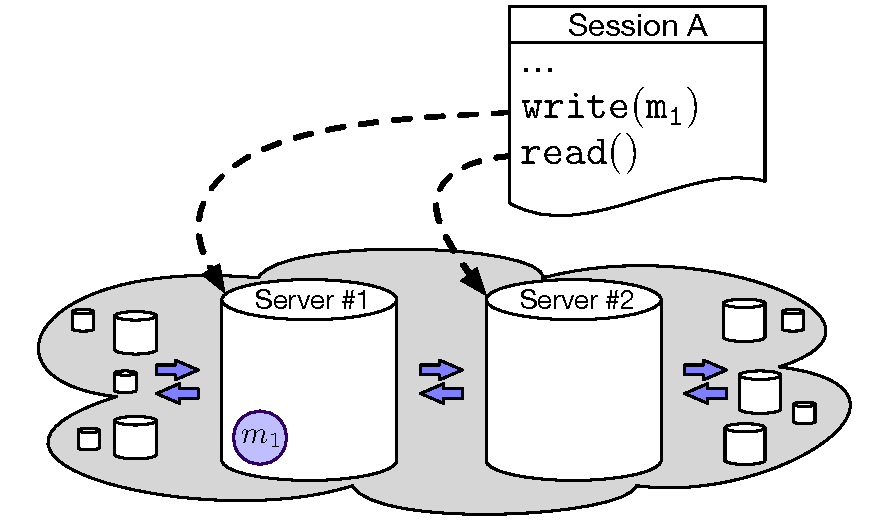
\includegraphics[scale=0.48]{../Figures/System_example.pdf}
\caption{A simple way of showing contracts}
\label{fig:ctrt}
\end{figure}


% Here, developers are forced to come up with their own implementation of
% RMW. They must modify client and server applications to generate, send
% and receive special tokens, to maintain the set of updates available at
% each server, and block user requests, if some necessary updates are
% still missing. Now, in order to have a correct application, the
% developer must prove certain non-trivial safety and liveness
% properties for this implementation. To make the matter worse, the
% proof will becmoe obsolete after each modification in the application or
% the consistency requirements. For example, after users reporting some unaccepatble
% behaviors, in order to disallow those executions, developers 
% implement and add another consistency guarantee to RMW; a task that
% would clearly make the original correctness proofs obsolete. 


% In this paper, we address these issues by introducing a compositional, principled approach to 
% derive enforcement mechanisms for various forms of weak consistency 
% guarantees. 
% We offer developers with a tool that generates a shim layer that works
% with an eventually consistent store and extends it to a key-value store
% with multiple environment, each of which shows a certain level of
% consistency, specified by the developers. 
% We also introduce a language for specifying application-level consistency 
% requirements as logical formulae that express legal execution states of the distributed store. 
% Our consistency enforcement methodology is independent of the underlying store 
% and only assumes the well-established guarantee of "eventual delivery". 
% Moreover, our enforcement tool is complete for the specification
% language, which itself is powerful enough to express all the known consistency 
% guarantees in the literature.

% We argue that all the consistency guarantees basically specify, \emph{when} an 
% application instance should block a user request and for arrival of 
% \emph{what} remote updates it should wait. For obvious reasons, any implementation of these 
% consistency guarantees must be \emph{correct} and \emph{optimal}. The former property states that 
% all possible behaviors of the implementation are allowed by the given specification and the later 
% ensures that application instances do not engage in 
% any unnecessary synchronization before responding to a user request (i.e. users are only blocked if 
% it is absolutely necessary).
% \\ Our technique is based on tracking relationships between update effects, and maintaining multiple 
% (logical) caches at the shim layer, each of which is enforced to satisfy a specific level of consistency, 
% derived from the given specifications. We believe that our approach is the first ever principled 
% reasoning and implementation framework for weak consistency enforcement techniques which 
% is also proven to be \emph{correct} and \emph{optimal}. 
% By separating all the consistency management procedures from the application level, we are taking 
% the non-trivial task of proving soundness criteria for ad-hoc consistency enforcement techniques 
% off of the developer's shoulders. 
% Contributions of the paper
A summary of our contributions is given below:
\begin{itemize}
  \item We propose a consistency specification language that lets
    programmers express the consistency requirements of their
    applications in terms of the dependencies between operations.

  \item We describe a generic consistency enforcement runtime that
    analyzes an operation's consistency specification, and ensures
    that its dependencies are satisfied before it is executed. We
    formalize the operational semantics of the runtime, and prove its
    correctness and optimality guarantees. Optimality includes
    \emph{minimum wait}, which guarantees that an operation waits (on
    arriving communication) only until its dependencies are satisfied,
    and \emph{minimum staleness}, which guarantees that among various
    states that satisfy an operation's dependencies, operation
    witnesses the latest state.
  
  \item We describe an implementation of our specification language and
    consistency enforcement runtime in a tool called \tool, which
    works on top of an off-the-shelf EC data store. We evaluate \tool
    over realistic applications and microbenchmarks, and present
    results that demonstrate the performance benefits of making
    fine-grained distinctions between consistency guarantees, and the
    ease of doing so via our specification language.

\end{itemize}

The remainder of the paper is organized as follows.  In Sec.
Sec.~\ref{sec:motivation} we provide additional motivation.
Sec.~\ref{sec:contract-lang} introduces the abstract store model that
forms the basis of our specification language, along with the language
itself.  We present a formal semantics of the consistency enforcement
runtime in Sec.~\ref{sec:formalization}, and provide correctness and
optimality guarantees. Sec.~\ref{sec:algorithm} elaborates on the
algorithmic aspects of our runtime that are key to its efficient
realization.  Sec.~\ref{sec:evaluation} describes \tool, an
implementation of the specification language and enforcement runtime,
and evaluates its applicability and practical utility.  Related work
and conclusions are presented in Sec.~\ref{sec:related-work}.
